% Provenance (never printed): old terminale S material on mountain ranges and
% continental collision (folds, reverse faults and nappes as signs of
% shortening and thickening; ophiolites and sutures as the trace of a closed
% ocean; the Himalaya and the Alps as examples). Owner (Sync 0): collision,
% fold/anticline/syncline/fold axis, reverse fault/thrust, nappe, ophiolite,
% suture, shortening. Fault is Book 1's (g7), normal fault g11.05's, the root
% and Airy isostasy g11.03's and g12.01's: recalled, never redefined. India's
% past latitudes: figdata/grade-12/india_drift.py (GPlates Web Service, two
% published plate models); shortening: figdata/grade-12/fold_shortening.py;
% the belt map: figdata/grade-12/alpine_belt.py.
\chapter{Gebergten bouwen}\label{ch:g12:mountain-building}

Klimmers die de top van de Mount Everest bereiken, \qty{8848.86}{m} boven
zeeniveau, staan op kalksteen. Geologen die monsters van de top
mee naar beneden namen, vonden erin brokstukken van trilobieten, mosselkreeftjes en
zeelelies: zeedieren die meer dan 440 miljoen jaar geleden leefden, in het
Ordovicium. Het hoogste gesteente ter wereld werd afgezet op de bodem van een
zee. Dit hoofdstuk legt uit hoe een zeebodem op het dak van de wereld belandt:
twee continenten botsen, en de korst ertussen wordt samengeperst, geplooid,
opgestapeld en verdikt tot een gebergteketen.
% ledger: sakai05:summit, tulane:roots (marine limestones at the top of Mt. Everest), ics:base.Ordovician, ics:base.Silurian (486.85-443.1 Ma); Book 1: tht:everest (8848.86 m)

\begin{omfigure}
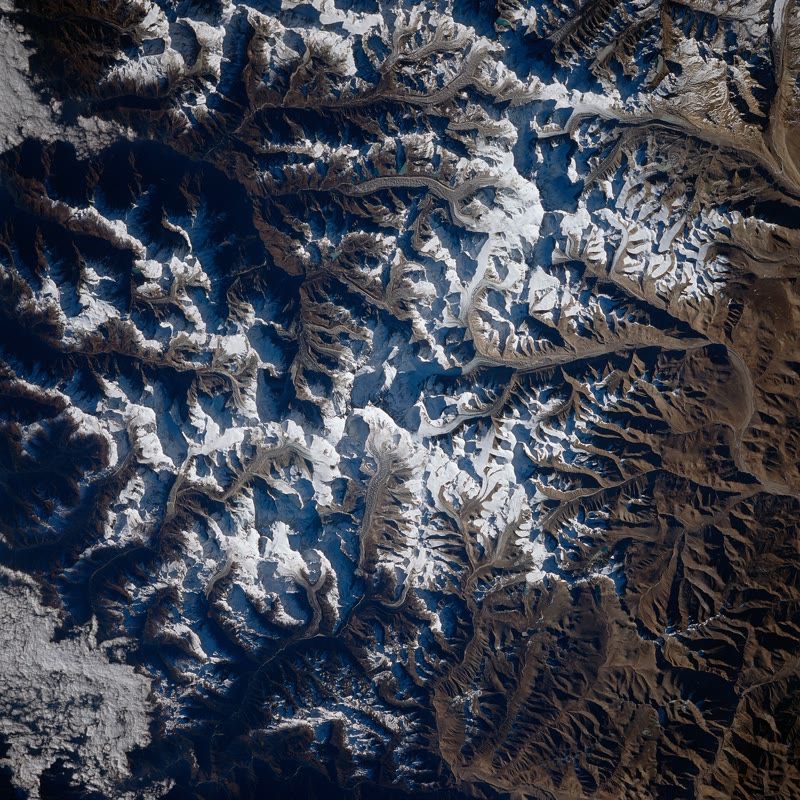
\includegraphics[width=0.5\linewidth]{images/book2/g12-nasa-everest-columbia.jpg}

{\small De Mount Everest en de vele gletsjers eromheen, gezien vanuit de
spaceshuttle Columbia op 30 november 1996. Foto NASA (publiek domein).}
\end{omfigure}
% ledger: photo:g12-everest-columbia

\begin{recall}
Een plaat \omterm{def:g11:ocean-ridges:oceanic-lithosphere}{oceanische lithosfeer}, gemaakt bij een rug, zinkt bij een trog terug in de
mantel; haar \omterm{def:g11:subduction-zones:slab}{slab} trekt haar omlaag (\cref{ch:g11:subduction-zones}). De
\omterm{def:g12:continental-crust:continental-crust}{continentale korst} is dik en licht, gemiddeld ongeveer \qty{2830}{kg/m^3}
tegen \qty{3380}{kg/m^3} voor de mantel eronder, dus ze drijft hoog, en een
dikke korst staat hoger dan een dunne, boven een \omterm{def:g12:continental-crust:root}{wortel}
(\cref{ch:g12:continental-crust,ch:g11:lithosphere-asthenosphere}). Een breuk
is een scheur waarlangs de twee blokken zijn verschoven; bij een \omterm{def:g11:ocean-ridges:normal-fault}{afschuiving} is het
blok boven het breukvlak omlaag gegaan, zoals waar de korst wordt uitgerekt
bij een trage rug (\cref{ch:g11:ocean-ridges}).
\end{recall}
% ledger: cm95:crust, data:prem, tulane:no-subduct, usgs:normal-fault

\section{Van subductie naar botsing}

Een oceaan die bij een trog sneller wordt verbruikt dan hij bij zijn rug wordt gemaakt,
krimpt. Een continent dat op de zinkende plaat meerijdt, komt met de snelheid van de
plaat dichter bij de trog, en ten slotte komt het er aan. De \omterm{def:g11:ocean-ridges:oceanic-lithosphere}{oceanische
lithosfeer} ervoor is naar beneden gegaan; het continent kan haar niet volgen,
omdat zijn korst te licht is om in de dichtere mantel te zinken. De \omterm{def:g11:subduction-zones:subduction}{subductie}
stopt. De twee continenten worden tegen elkaar geperst, en de \omterm{def:g11:subduction-zones:slab}{slab}
die aan de oceaanbodem hing, breekt uiteindelijk af en zinkt in de
mantel.
% ledger: earle:collision, tulane:no-subduct

\begin{definition}[Continentale botsing]\label{def:g12:mountain-building:collision}
Een \emph{continentale botsing}\index{continentale botsing} is de ontmoeting van
twee continenten aan een convergente plaatgrens, nadat de \omterm{def:g11:ocean-ridges:oceanic-lithosphere}{oceanische lithosfeer}
ertussen is gesubduceerd. Geen van beide continenten zinkt: de korst ertussen
wordt vervormd en verdikt tot een gebergtegordel.
\end{definition}
% ledger: earle:collision, tulane:no-subduct, usgs:himalaya-collision

\begin{omfigure}
\begin{tikzpicture}[x=0.95cm, y=0.95cm, font=\scriptsize]
  % ---- stage 1: the ocean closes ----
  \begin{scope}[yshift=0cm]
    \fill[omSea] (3.4,0) -- (8.6,0) -- (8.0,-0.5) -- (4.3,-0.5) -- (3.5,0.0) -- cycle;
    \fill[omLithGranite] (0,0.15) -- (3.5,0.15) -- (4.3,-0.5) -- (4.3,-0.75) -- (3.5,-1.0) -- (0,-1.0) -- cycle;
    \fill[omLithBasalt] (4.3,-0.5) -- (8.0,-0.5) .. controls (9.0,-0.75) and (9.6,-1.2) .. (10.4,-2.0)
      -- (10.15,-2.15) .. controls (9.4,-1.4) and (8.9,-1.0) .. (8.0,-0.75) -- (4.3,-0.75) -- cycle;
    \fill[omLithGranite] (8.0,-0.5) -- (8.6,0.2) -- (12,0.2) -- (12,-1.05) -- (9.5,-1.05)
      .. controls (9.0,-0.75) .. (8.0,-0.5) -- cycle;
    \fill[omThm!70] (10.0,0.2) -- (10.3,0.55) -- (10.6,0.2) -- cycle;
    \draw[black!60, line width=0.3pt] (0,0.15) -- (3.5,0.15) -- (4.3,-0.5) -- (8.0,-0.5) -- (8.6,0.2) -- (12,0.2);
    \draw[-{Stealth[length=2mm]}, line width=0.8pt] (1.2,0.45) -- (2.6,0.45);
    \node[anchor=east] at (0,-0.4) {1};
    \node at (1.8,-0.5) {continent};
    \node at (6.1,-0.25) {oceaan};
    \node[anchor=north] at (6.1,-0.8) {oceanische lithosfeer};
    \node[anchor=south] at (8.0,0.0) {trog};
    \node[anchor=south] at (10.3,0.55) {vulkanische boog};
    \node at (11.1,-0.5) {continent};
  \end{scope}
  % ---- stage 2: the continents meet ----
  \begin{scope}[yshift=-3.0cm]
    \fill[omSea] (6.9,0) -- (8.4,0) -- (8.0,-0.4) -- (7.4,-0.35) -- cycle;
    \fill[omLithGranite] (0,0.15) -- (6.8,0.15) -- (7.6,-0.4) -- (8.0,-0.5)
      .. controls (9.0,-0.75) .. (9.5,-1.05) -- (9.2,-1.4) -- (6.5,-1.0) -- (0,-1.0) -- cycle;
    \fill[omLithBasalt] (9.5,-1.05) .. controls (10.0,-1.4) .. (10.6,-2.0) -- (10.35,-2.15)
      .. controls (9.8,-1.6) .. (9.2,-1.4) -- cycle;
    \fill[omLithGranite] (8.0,-0.5) -- (8.6,0.2) -- (12,0.2) -- (12,-1.05) -- (9.5,-1.05)
      .. controls (9.0,-0.75) .. (8.0,-0.5) -- cycle;
    \fill[omLithPeridotite] (7.0,0.15) -- (7.9,0.15) -- (8.3,0.05) -- (7.95,-0.12) -- (7.3,0.0) -- cycle;
    \fill[omThm!70] (10.0,0.2) -- (10.3,0.55) -- (10.6,0.2) -- cycle;
    \draw[-{Stealth[length=2mm]}, line width=0.8pt] (3.2,0.45) -- (4.6,0.45);
    \node[anchor=east] at (0,-0.4) {2};
    \node at (3.4,-0.45) {continent};
    \draw[black!60] (7.6,0.12) -- (7.0,0.75) node[anchor=south east, inner sep=1pt] {schijf oceaanbodem};
    \node at (11.1,-0.5) {continent};
    \node[anchor=west] at (10.7,-1.9) {slab};
  \end{scope}
  % ---- stage 3: a mountain belt ----
  \begin{scope}[yshift=-6.4cm]
    \fill[omLithGranite] (0,0.15) -- (4.5,0.15) .. controls (6.0,0.4) and (6.6,1.25) .. (7.6,1.3)
      .. controls (8.7,1.3) and (9.6,0.5) .. (10.6,0.2) -- (12,0.2) -- (12,-1.05) -- (10.6,-1.1)
      .. controls (9.5,-2.2) and (8.6,-2.6) .. (7.7,-2.6) .. controls (6.6,-2.6) and (5.6,-1.6) .. (4.5,-1.0)
      -- (0,-1.0) -- cycle;
    \draw[black!60, line width=0.3pt] (0,0.15) -- (4.5,0.15) .. controls (6.0,0.4) and (6.6,1.25) .. (7.6,1.3)
      .. controls (8.7,1.3) and (9.6,0.5) .. (10.6,0.2) -- (12,0.2);
    \draw[black!60, dashed, line width=0.4pt] (0,-1.0) -- (4.5,-1.0) .. controls (5.6,-1.6) and (6.6,-2.6) .. (7.7,-2.6)
      .. controls (8.6,-2.6) and (9.5,-2.2) .. (10.6,-1.1) -- (12,-1.05);
    \draw[omThm, line width=1.0pt] (7.0,1.25) -- (8.3,-2.55);
    \foreach \t in {0.15,0.4,0.65}
      \fill[omLithPeridotite] ($(7.0,1.25)!\t!(8.3,-2.55)$) ++(-0.12,0.05) -- ++(0.3,0) -- ++(-0.05,-0.22) -- ++(-0.3,0) -- cycle;
    \fill[omLithBasalt] (10.9,-1.9) -- (11.5,-2.35) -- (11.35,-2.5) -- (10.75,-2.05) -- cycle;
    \node[anchor=east] at (0,-0.4) {3};
    \node at (2.4,-0.45) {continent};
    \node at (11.3,-0.5) {continent};
    \draw[black!60] (7.2,0.6) -- (5.9,1.5) node[anchor=east, inner sep=1pt] {sutuur met ofiolieten};
    \node at (7.7,-1.9) {wortel};
    \node[anchor=north] at (11.2,-2.5) {afgebroken slab};
    \node[anchor=south] at (7.6,1.35) {gebergtegordel};
  \end{scope}
\end{tikzpicture}

{\small Van \omterm{def:g11:subduction-zones:subduction}{subductie} naar botsing (niet op schaal). 1: een oceaan sluit zich terwijl
zijn bodem bij een trog zinkt. 2: het continent komt bij de trog aan en
kan niet zinken; schijven oceaanbodem worden op zijn rand geschoven. 3: de korst
tussen de twee continenten wordt verkort en verdikt tot een gebergtegordel
die boven een \omterm{def:g12:continental-crust:root}{wortel} staat; de lijn waar de twee continenten aan elkaar vastzitten, gemarkeerd
door schijven oceaanbodem, is de \omterm{def:g12:mountain-building:suture}{sutuur}; de \omterm{def:g11:subduction-zones:slab}{slab} breekt af en zinkt.}
\end{omfigure}
% ledger: earle:collision, tulane:ocean-basins, usgs:suture, tulane:roots

\subsection{Het spoor van een verdwenen oceaan}

Wanneer de oceaan zich heeft gesloten, zijn de twee continenten langs een lijn aan elkaar gelast.

\begin{definition}[Sutuur]\label{def:g12:mountain-building:suture}
Een \emph{sutuur}\index{sutuur} is de lijn, of smalle zone, waarlangs twee
continenten door een botsing aan elkaar zijn gevoegd, nadat de \omterm{def:g11:subduction-zones:subduction}{subductie} ertussen
is gestopt: het spoor van een vroegere plaatgrens. Ze markeert waar de oceaan
ertussen vroeger lag.
\end{definition}
% ledger: usgs:suture, liu20:itsz

Wat markeert een \omterm{def:g12:mountain-building:suture}{sutuur}? Langs veel suturen liggen gesteentelichamen die
nergens op een continent thuishoren: van boven naar beneden mariene sedimenten,
kussenbasalten, een massa verticale \omterm{def:g11:igneous-rocks:intrusion}{gangen} die naast elkaar staan, \omterm{def:g11:ocean-ridges:gabbro}{gabbro}, en aan de
basis \omterm{def:g11:ocean-ridges:peridotite}{peridotiet} van de mantel: de lagen van de oceaanbodem
(\cref{ch:g11:ocean-ridges}), met de top van de mantel eronder.
% ledger: tulane:ocean-basins

\begin{definition}[Ofioliet]\label{def:g12:mountain-building:ophiolite}
Een \emph{ofioliet}\index{ofioliet} is een stuk \omterm{def:g11:ocean-ridges:oceanic-lithosphere}{oceanische lithosfeer} ---
sedimenten, kussenbasalten, gangencomplex, \omterm{def:g11:ocean-ridges:gabbro}{gabbro} en mantelperidotiet ---
dat op \omterm{def:g12:continental-crust:continental-crust}{continentale korst} is geschoven.
\end{definition}
% ledger: tulane:ocean-basins

Een \omterm{def:g12:mountain-building:ophiolite}{ofioliet} is gestrande oceaanbodem: een schijf van de verdwenen oceaan, op een
continent geschoven in plaats van met de rest te zinken. De gebergten die door
een botsing worden opgeworpen, bevatten vaak wat oceaankorst en bovenmantel, omdat daar
een oceaan zich sloot. In het zuiden van Tibet zijn de \omterm{def:g12:mountain-building:ophiolite}{ofiolieten} die
langs de Indus--Tsangpo-sutuur zijn aaneengeregen, resten van een oceaan die de
Neo-Tethys heet en die tussen India en de streek van Lhasa lag; een \omterm{def:g11:ocean-ridges:gabbro}{gabbro} daar
is gedateerd op 243 miljoen jaar.
% ledger: tulane:ocean-basins, earle:collision, liu20:itsz

\begin{omfigure}
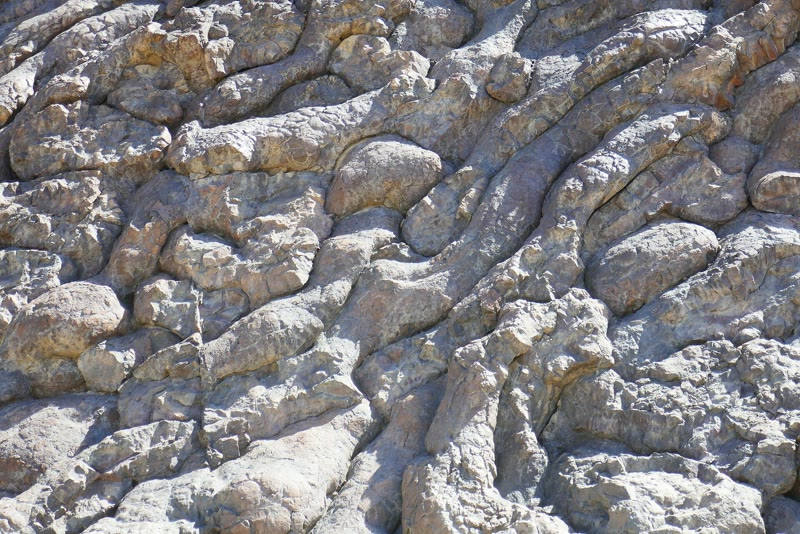
\includegraphics[width=0.6\linewidth]{images/book2/g12-duchoiselle-oman-pillows.jpg}

{\small Kussenlava van de \omterm{def:g12:mountain-building:ophiolite}{ofioliet} van Semail bij Wadi Jizzi, Oman: lava die
onder water afkoelde tot ronde kussens, nu op het land. Foto Lionel
Duchoiselle (CC~BY-SA~3.0).}
\end{omfigure}
% ledger: photo:g12-oman-pillows

\section{De korst verkorten}

Van opzij samengeperst breekt een gesteentelichaam als het koud en bros is; als
het warm genoeg is om zich plastisch te gedragen, plooit het. Een gebergtegordel zit
vol \omterm{def:g12:mountain-building:fold}{plooien} en breuken.
% ledger: earle:folds

\subsection{Plooien}

\begin{definition}[Plooi; anticlinaal; synclinaal; plooias]\label{def:g12:mountain-building:fold}
Een \emph{plooi}\index{plooi} is een buiging in gesteentelagen. Haar hellende zijden zijn
de \emph{flanken}; ze ontmoeten elkaar in het \emph{scharnier}, waar de lagen het sterkst
gekromd zijn, en de lijn langs het scharnier is de
\emph{plooias}\index{plooias}. Een \emph{anticlinaal}\index{anticlinaal} is een plooi waarvan de lagen
naar boven buigen, met flanken die van de as af hellen; een
\emph{synclinaal}\index{synclinaal} is een plooi waarvan de lagen naar beneden buigen, met
flanken die naar de as toe hellen.
\end{definition}
% ledger: earle:folds, tulane:fold-geometry

Het vlak door de scharnieren van de opeenvolgende lagen is het assenvlak.
Anticlinalen en synclinalen komen meestal in paren voor, waarbij de flank van de ene de
flank van de volgende is. \omterm{def:g12:mountain-building:fold}{Plooien} komen in elke grootte voor, van microscopisch tot tientallen
kilometers breed. Eenmaal geërodeerd toont een \omterm{def:g12:mountain-building:fold}{anticlinaal} zijn oudste lagen in
zijn kern en een \omterm{def:g12:mountain-building:fold}{synclinaal} zijn jongste; een \omterm{def:g12:mountain-building:fold}{anticlinaal} is niet noodzakelijk een
rug, en een \omterm{def:g12:mountain-building:fold}{synclinaal} niet noodzakelijk een dal, omdat erosie de harde en de
zachte lagen volgt in plaats van de vorm van de \omterm{def:g12:mountain-building:fold}{plooi}.
% ledger: earle:folds, tulane:fold-geometry

\begin{omfigure}
\begin{tikzpicture}[x=1.2cm, y=1.2cm, font=\scriptsize]
  \def\W{6}\def\H{2.0}\def\dx{1.35}\def\dy{0.78}
  \tikzset{declare function={zb(\x,\c)=\c+0.8*cos(60*(\x-1.5));}}
  \colorlet{bandA}{omLithSchist!70}\colorlet{bandB}{omLithSand}\colorlet{bandC}{omLithShale}
  \colorlet{bandD}{icsJurassic!35}\colorlet{bandE}{icsTriassic!35}\colorlet{bandF}{icsCretaceous!45}
  % front face
  \begin{scope}
    \clip (0,0) rectangle (\W,\H);
    \fill[bandA] (0,0) rectangle (\W,\H);
    \foreach \c/\col in {0.0/bandB, 0.6/bandC, 1.2/bandD, 1.8/bandE, 2.4/bandF}
      \fill[\col] plot[domain=0:\W, samples=80, smooth] (\x,{zb(\x,\c)}) -- (\W,4) -- (0,4) -- cycle;
    \foreach \c in {0.0,0.6,1.2,1.8,2.4}
      \draw[black!55, line width=0.35pt] plot[domain=0:\W, samples=80, smooth] (\x,{zb(\x,\c)});
  \end{scope}
  % top face: outcrop bands (crossings of the top surface computed for these curves)
  \fill[bandE] (0,\H) -- (0.242,\H) -- ++(\dx,\dy) -- (\dx,\H+\dy) -- cycle;
  \fill[bandD] (0.242,\H) -- (2.758,\H) -- ++(\dx,\dy) -- (0.242+\dx,\H+\dy) -- cycle;
  \fill[bandE] (2.758,\H) -- (3.5,\H) -- ++(\dx,\dy) -- (2.758+\dx,\H+\dy) -- cycle;
  \fill[bandF] (3.5,\H) -- (5.5,\H) -- ++(\dx,\dy) -- (3.5+\dx,\H+\dy) -- cycle;
  \fill[bandE] (5.5,\H) -- (\W,\H) -- ++(\dx,\dy) -- (5.5+\dx,\H+\dy) -- cycle;
  \foreach \x in {0.242,2.758,3.5,5.5} \draw[black!55, line width=0.35pt] (\x,\H) -- ++(\dx,\dy);
  % right face: the layers meet it at constant heights (cylindrical folds)
  \foreach \lo/\hi/\col in {0.0/0.6/bandB, 0.6/1.2/bandC, 1.2/1.8/bandD, 1.8/2.0/bandE}
    \fill[\col] (\W,\lo) -- (\W+\dx,\lo+\dy) -- (\W+\dx,\hi+\dy) -- (\W,\hi) -- cycle;
  \foreach \y in {0.6,1.2,1.8} \draw[black!55, line width=0.35pt] (\W,\y) -- ++(\dx,\dy);
  % outline
  \draw[black, line width=0.5pt] (0,0) rectangle (\W,\H) (0,\H) -- (\dx,\H+\dy) -- (\W+\dx,\H+\dy) -- (\W,\H)
    (\W+\dx,\H+\dy) -- (\W+\dx,\dy) -- (\W,0);
  % fold axes on the top face, axial planes on the front face
  \draw[omThm, line width=1pt] (1.5,\H) -- ++(\dx,\dy);
  \draw[omDef, line width=1pt] (4.5,\H) -- ++(\dx,\dy);
  \draw[omThm, dashed, line width=0.6pt] (1.5,0) -- (1.5,\H);
  \draw[omDef, dashed, line width=0.6pt] (4.5,0) -- (4.5,\H);
  \node[anchor=south, omThm] at (1.5+\dx,\H+\dy) {anticlinaal: plooias};
  \node[anchor=south, omDef] at (4.5+\dx,\H+\dy) {synclinaal: plooias};
  \draw[black!70] (3.2,0.95) -- (3.9,-0.35) node[anchor=north] {flank};
  \draw[black!70] (1.5,1.4) circle (0.07) -- (0.4,-0.35) node[anchor=north] {scharnier};
  \draw[black!70] (1.5,0.25) -- (2.0,-0.35) node[anchor=north] {assenvlak};
\end{tikzpicture}

{\small Een \omterm{def:g12:mountain-building:fold}{anticlinaal} en een \omterm{def:g12:mountain-building:fold}{synclinaal}, afgesneden door een vlak erosieoppervlak
(blokdiagram, niet op schaal). De plooiassen lopen langs de scharnieren; de gestreepte
lijnen zijn de sporen van de assenvlakken. Aan het bovenvlak toont de geërodeerde
\omterm{def:g12:mountain-building:fold}{anticlinaal} oudere lagen in zijn kern, de \omterm{def:g12:mountain-building:fold}{synclinaal} jongere.}
\end{omfigure}
% ledger: earle:folds, tulane:fold-geometry

\begin{omfigure}
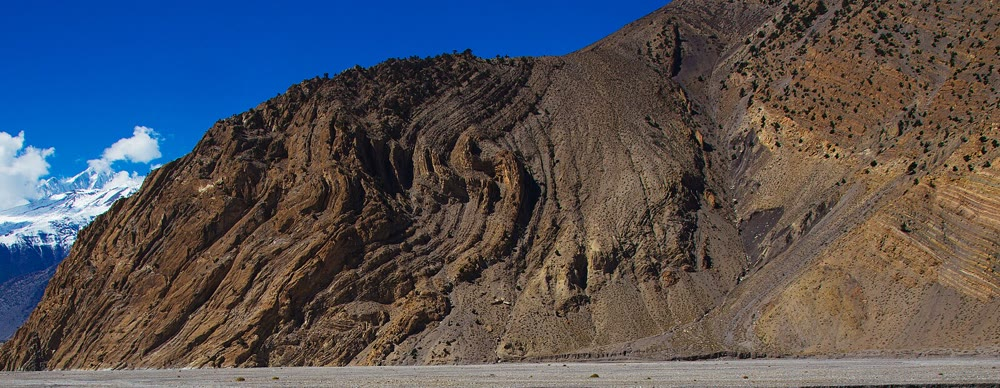
\includegraphics[width=0.95\linewidth]{images/book2/g12-hullot-kali-gandaki-folds.jpg}

{\small Geplooide gesteentelagen in een rotswand van de Himalaya, ongeveer
\qty{3}{km} ten noordoosten van Jomsom in de kloof van de Kali Gandaki, Nepal.
Foto Jean-Marie Hullot (CC~BY~2.0).}
\end{omfigure}
% ledger: photo:g12-kali-gandaki

De bedekking van de Varden Hills is op dezelfde manier geplooid, maar veel zachter.
Haar zandsteen, kalksteen, schalie en krijt werden vlak afgezet en daarna gebogen
tot een \omterm{def:g12:mountain-building:fold}{anticlinaal} en een \omterm{def:g12:mountain-building:fold}{synclinaal} waarvan de flanken \ang{12} hellen; een latere
\omterm{def:g11:ocean-ridges:normal-fault}{afschuiving} snijdt ze af.
% ledger: region:name; model in figdata/shared/region.py (LIMB_DIP 12, AXIS_ANTI 3.5 km, AXIS_SYN 7.5 km)

\begin{omfigure}
\begin{tikzpicture}
\begin{axis}[omsection, x=1.25cm, y=0.003125cm, xmin=0, xmax=9.49, ymin=-700, ymax=650,
  xlabel={afstand vanaf A (\unit{km})}, ylabel={hoogte (\unit{m})},
  ytick={-600,-300,0,300,600}, tick label style={font=\scriptsize}]
\addplot[fill=black!8, draw=black!50, line width=0.3pt, even odd rule] table {figdata/out/shared-region-section-unit-schist.dat};
\addplot[fill=icsTriassic!20, draw=black!50, line width=0.3pt, even odd rule] table {figdata/out/shared-region-section-unit-sandstone.dat};
\addplot[fill=icsJurassic!25, draw=black!50, line width=0.3pt, even odd rule] table {figdata/out/shared-region-section-unit-limestone.dat};
\addplot[fill=icsJurassic!8, draw=black!50, line width=0.3pt, even odd rule] table {figdata/out/shared-region-section-unit-shale.dat};
\addplot[fill=icsCretaceous!20, draw=black!50, line width=0.3pt, even odd rule] table {figdata/out/shared-region-section-unit-chalk.dat};
\addplot[fill=omLithAlluv, draw=black!50, line width=0.3pt, even odd rule] table {figdata/out/shared-region-section-unit-alluvium.dat};
\addplot[black, line width=0.7pt] table {figdata/out/shared-region-section-ground.dat};
\addplot[fault] table {figdata/out/shared-region-section-fault.dat};
% axis positions from figdata/grade-12/fold_shortening.py (section_anticline_km, section_syncline_km; the syncline lies on the hanging wall, shifted by the fault heave)
\draw[omThm, dashed, line width=0.7pt] (axis cs:3.162,-700) -- (axis cs:3.162,660);
\draw[omDef, dashed, line width=0.7pt] (axis cs:7.484,-700) -- (axis cs:7.484,660);
\node[anchor=south, omThm, font=\scriptsize] at (axis cs:3.162,660) {as van de anticlinaal};
\node[anchor=south, omDef, font=\scriptsize] at (axis cs:7.484,660) {as van de synclinaal};
\node[anchor=south east, font=\small\bfseries] at (axis cs:0,650) {A};
\node[anchor=south west, font=\small\bfseries] at (axis cs:9.49,650) {B};
\node[font=\scriptsize, fill=white, inner sep=1pt] at (axis cs:1.2,-520) {schist};
\node[font=\scriptsize, fill=white, inner sep=1pt, anchor=east] at (axis cs:6.55,-450) {afschuiving};
\end{axis}
\end{tikzpicture}

\smallskip
{\small\tikz\fill[black!8, draw=black!50] (0,0) rectangle (0.35,0.22);~schist \quad
\tikz\fill[icsTriassic!20, draw=black!50] (0,0) rectangle (0.35,0.22);~zandsteen \quad
\tikz\fill[icsJurassic!25, draw=black!50] (0,0) rectangle (0.35,0.22);~kalksteen \quad
\tikz\fill[icsJurassic!8, draw=black!50] (0,0) rectangle (0.35,0.22);~schalie \quad
\tikz\fill[icsCretaceous!20, draw=black!50] (0,0) rectangle (0.35,0.22);~krijt \quad
\omve{2.5}}

{\small Doorsnede A--B door de Varden Hills, van het zuidwesten naar het
noordoosten. De bedekking rust op de sokkel van schist en is geplooid tot een
\omterm{def:g12:mountain-building:fold}{anticlinaal} en een \omterm{def:g12:mountain-building:fold}{synclinaal}; de \omterm{def:g11:ocean-ridges:normal-fault}{afschuiving}, jonger dan de \omterm{def:g12:mountain-building:fold}{plooien}, laat
het noordoostelijke blok zakken. De verticale schaal is 2.5 keer uitgerekt, waardoor
de flanken steiler lijken dan ze zijn. Gegevens: het model van de reeks voor de
streek.}
\end{omfigure}
% ledger: region:name; computed in figdata/shared/region.py (section A-B)

\subsection{Opschuivingen, overschuivingen en dekbladen}

Waar de korst wordt samengeperst terwijl ze koud en bros is, breekt ze langs breuken
van een andere soort dan de \omterm{def:g11:ocean-ridges:normal-fault}{afschuivingen} van uitgerekte korst.

\begin{definition}[Opschuiving; overschuiving]\label{def:g12:mountain-building:thrust}
Een \emph{opschuiving}\index{opschuiving} is een hellende breuk waarlangs
het blok boven het breukvlak omhoog is gegaan ten opzichte van het blok
eronder. Opschuivingen ontstaan waar de korst wordt samengeperst. Een
\emph{overschuiving}\index{overschuiving} is een opschuiving met een flauwe helling, minder dan
\ang{45}.
\end{definition}
% ledger: earle:reverse-thrust, tulane:fold-geometry

Een \omterm{def:g12:mountain-building:thrust}{overschuiving} kan een gesteenteplaat tientallen kilometers ver dragen, en dan komen oudere
gesteenten boven op jongere te liggen, tegen de volgorde in waarin ze
zijn afgezet. In de Rocky Mountains heeft de McConnell-overschuiving een
stapel sedimentaire gesteenten van ongeveer \qty{800}{m} dik zo'n \qty{40}{km} van
west naar oost geschoven: kalksteen van ongeveer 500 miljoen jaar oud ligt nu op een kleisteen
van ongeveer 75 miljoen jaar oud.
% ledger: earle:reverse-thrust

\begin{definition}[Dekblad]\label{def:g12:mountain-building:nappe}
Een \emph{dekblad}\index{dekblad} is een grote gesteenteplaat die over een
grote afstand, vaak tientallen kilometers, over de gesteenten eronder is gedragen langs een
\omterm{def:g12:mountain-building:thrust}{overschuiving} die bijna vlak is.
\end{definition}
% ledger: ngu:nappe, earle:reverse-thrust

Een \omterm{def:g12:mountain-building:nappe}{dekblad} kan gesteenten dragen die ver weg zijn ontstaan, zelfs schijven oceaanbodem; het
kan zelf geplooid zijn, met omgekeerde lagen. Gebergtegordels stapelen \omterm{def:g12:mountain-building:nappe}{dekbladen}
op elkaar. Erosie snijdt later gaten door een \omterm{def:g12:mountain-building:nappe}{dekblad}, die
vensters openen op de gesteenten eronder, en laat er losse stukken van achter op
de jongere gesteenten.
% ledger: ngu:nappe

\begin{omfigure}
\begin{tikzpicture}[x=1.0cm, y=1.0cm, font=\scriptsize]
  % rocks in place (younger), flat-lying
  \fill[icsCretaceous!25] (0,-1.6) rectangle (12,-0.4);
  \fill[icsJurassic!25] (0,-1.6) rectangle (12,-1.1);
  \draw[black!50, line width=0.3pt] (0,-1.1) -- (12,-1.1);
  \fill[white] (5.6,-0.4) -- (6.2,-0.62) -- (6.8,-0.4) -- cycle;
  % the nappe (older rocks) above a nearly flat thrust, cut by erosion
  \fill[omLithSchist!80] (0.8,-0.4) .. controls (1.2,0.35) and (1.9,0.35) .. (2.3,-0.4) -- cycle;
  \fill[omLithSchist!80] (3.2,-0.4) .. controls (3.9,0.9) and (4.8,0.9) .. (5.6,-0.4) -- cycle;
  \fill[omLithSchist!80] (6.8,-0.4) .. controls (7.1,0.9) and (7.7,1.3) .. (8.4,1.25) -- (12,0.9) -- (12,-0.4) -- cycle;
  % ground surface
  \draw[black, line width=0.6pt] (0,-0.4) -- (0.8,-0.4) .. controls (1.2,0.35) and (1.9,0.35) .. (2.3,-0.4)
     -- (3.2,-0.4) .. controls (3.9,0.9) and (4.8,0.9) .. (5.6,-0.4) -- (6.2,-0.62) -- (6.8,-0.4)
     .. controls (7.1,0.9) and (7.7,1.3) .. (8.4,1.25) -- (12,0.9);
  % thrust traces (teeth on the block that moved over)
  \draw[thrust fault] (0.8,-0.4) -- (2.3,-0.4);
  \draw[thrust fault] (3.2,-0.4) -- (5.6,-0.4);
  \draw[thrust fault] (6.8,-0.4) -- (12,-0.4);
  \draw[-{Stealth[length=2mm]}, line width=0.9pt] (11.4,1.45) -- (9.6,1.6);
  \node[anchor=south] at (10.5,1.55) {beweging van het dekblad};
  \node at (9.9,0.3) {dekblad: oudere gesteenten};
  \node[fill=white, inner sep=1pt] at (2.0,-0.85) {gesteenten ter plaatse: jonger};
  \draw[black!60] (1.55,0.0) -- (1.3,0.8) node[anchor=south] {los stuk};
  \draw[black!60] (6.2,-0.58) -- (6.2,-0.68) node[anchor=north, fill=white, inner sep=1pt] {venster};
  \draw[black!60] (9.0,-0.42) -- (9.3,-0.68) node[anchor=north, fill=white, inner sep=1pt] {overschuiving};
\end{tikzpicture}

{\small Een \omterm{def:g12:mountain-building:nappe}{dekblad} (niet op schaal): een plaat oudere gesteenten die langs een
bijna vlakke \omterm{def:g12:mountain-building:thrust}{overschuiving} is gedragen over jongere gesteenten die ter plaatse zijn gebleven. Erosie heeft
er een venster door gesneden en links een los stuk ervan achtergelaten. De
tanden op de \omterm{def:g12:mountain-building:thrust}{overschuiving} wijzen naar het blok dat eroverheen schoof.}
\end{omfigure}
% ledger: ngu:nappe, earle:reverse-thrust

\begin{omfigure}
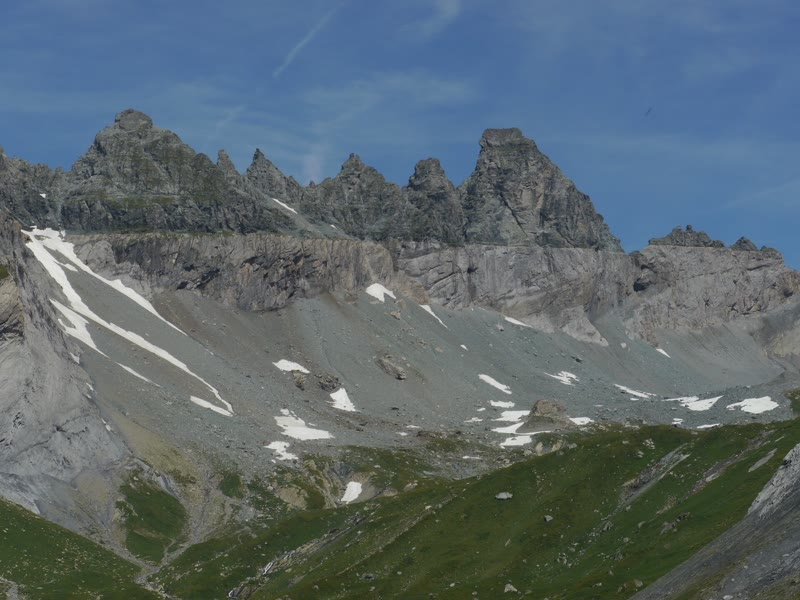
\includegraphics[width=0.5\linewidth]{images/book2/g12-heine-glarus-thrust.jpg}

{\small De Glarus-overschuiving in de Alpen van Oost-Zwitserland. De donkere
gesteenten van de toppen, afgezet in het Perm, tussen ongeveer 299 en 252
miljoen jaar geleden, rusten op lichtere en veel jongere gesteenten; de \omterm{def:g12:mountain-building:thrust}{overschuiving} is de
scherpe grens ertussen. De bovenste gesteenten zijn zo'n 40 tot
\qty{50}{km} verschoven. Foto Christian Heine (CC~BY-SA~3.0).}
\end{omfigure}
% ledger: photo:g12-glarus (Verrucano, Permian; displacement 40-50 km, Pfiffner 1985), ics:base.Permian, ics:base.Triassic

\subsection{De verkorting meten}

\omterm{def:g12:mountain-building:fold}{Plooien} en \omterm{def:g12:mountain-building:thrust}{overschuivingen} maken de korst allebei korter in de richting waarin ze wordt
samengeperst.

\begin{definition}[Verkorting]\label{def:g12:mountain-building:shortening}
De \emph{verkorting}\index{verkorting} van een laag is het deel van haar
lengte dat ze heeft verloren: als ze $L_0$ lang was en nu $L$ overspant,
\[
  e = \frac{L_0 - L}{L_0}.
\]
\end{definition}

Om haar te meten heb je de oorspronkelijke lengte $L_0$ nodig. In veel \omterm{def:g12:mountain-building:fold}{plooien} behouden de
lagen hun dikte terwijl ze buigen, en glijden ze over elkaar zoals de
bladzijden van een gebogen boek; zo'n laag wordt in haar lengte niet uitgerekt. Dat
geeft de oorspronkelijke lengte.
% ledger: tulane:fold-geometry (flexural folds keep their thickness)

\begin{proposition}[De verkorting van een geplooide laag]\label{prop:g12:mountain-building:shortening}
Als een laag is geplooid zonder in haar eigen richting te worden uitgerekt of samengeperst,
is haar oorspronkelijke lengte $L_0$ haar lengte gemeten langs de geplooide laag.
Voor een \omterm{def:g12:mountain-building:fold}{plooi} met rechte flanken die onder een hoek $\theta$ hellen, geldt
\[
  e = 1 - \cos\theta .
\]
\end{proposition}

\begin{proof}
Wie de laag ontplooit zonder haar uit te rekken, legt haar vlak neer met
ongewijzigde lengte; dus is $L_0$ de lengte langs de laag. Op een rechte
flank met lengte $\ell$ die onder $\theta$ helt, is de afgelegde horizontale afstand
$\ell\cos\theta$ (rechthoekige driehoek). Telt men alle flanken op, dan overspant de laag met
lengte $L_0$ een afstand $L = L_0\cos\theta$, en $e = (L_0 - L_0\cos\theta)/L_0 =
1 - \cos\theta$.
\end{proof}

\begin{omfigure}
\begin{tikzpicture}
\begin{axis}[name=sine, x=2.0cm, y=2.0cm, axis lines=none,
  xmin=-0.05, xmax=2.25, ymin=-0.4, ymax=0.8, clip=false]
% computed in figdata/grade-12/fold_shortening.py (part sine: A/lambda = 0.25, e = 31.7 %)
\addplot[omLithSand!80!black, line width=1.6pt] table[x=x, y=y] {figdata/out/grade-12-fold_shortening-sine.dat};
\draw[omThm, line width=1.6pt] (axis cs:0,0.62) -- (axis cs:2.196,0.62);
\draw[black!60, |-|] (axis cs:0,-0.32) -- node[below, font=\scriptsize] {$L$ (vandaag)} (axis cs:1.5,-0.32);
\node[anchor=south west, font=\scriptsize, omThm] at (axis cs:0,0.64) {$L_0$: dezelfde laag ontplooid};
\end{axis}
\begin{axis}[omrecord, at={(sine.east)}, anchor=west, xshift=1.4cm, width=0.46\linewidth, height=4.6cm,
  xmin=0, xmax=80, ymin=0, ymax=85, xlabel={helling van de flank $\theta$ (\unit{\degree})},
  ylabel={verkorting $e$ (\unit{\percent})}, xtick={0,20,...,80}]
% computed in figdata/grade-12/fold_shortening.py (part dip: e = 1 - cos theta)
\addplot[omProp, line width=1pt] table[x=theta, y=e_pct] {figdata/out/grade-12-fold_shortening-dip.dat};
\addplot[only marks, mark=*, mark size=1.6pt, omThm] coordinates {(12,2.185) (30,13.397) (60,50)};
\node[anchor=south, font=\scriptsize, align=center] at (axis cs:12,6) {Varden:\\\qty{2.2}{\percent}};
\node[anchor=west, font=\scriptsize] at (axis cs:32,10) {\qty{13}{\percent}};
\node[anchor=south east, font=\scriptsize] at (axis cs:60,51) {\qty{50}{\percent}};
\end{axis}
\end{tikzpicture}

{\small Links: een geplooide laag overspant $L$; vlak neergelegd, zonder te worden
uitgerekt, is ze $L_0$ lang (hier zijn de \omterm{def:g12:mountain-building:fold}{plooien} zo hoog als een kwart van
hun golflengte, en is $L$ \qty{68}{\percent} van $L_0$). Rechts: de
\omterm{def:g12:mountain-building:shortening}{verkorting} van een \omterm{def:g12:mountain-building:fold}{plooi} met rechte flanken, $1 - \cos\theta$, tegen de helling
van haar flanken. Zachte \omterm{def:g12:mountain-building:fold}{plooien} verkorten een laag maar heel weinig.}
\end{omfigure}
% values: sine_025_e_pct 31.68 (L/L0 = 0.683); varden_e_pct 2.1852; chevron_30 13.397; chevron_60 50 (fold_shortening.py)

\begin{method}[De verkorting meten op een doorsnede]\label{met:g12:mountain-building:shortening}
\begin{enumerate}
  \item Controleer of de doorsnede op ware schaal is getekend. Als haar verticale schaal
        is uitgerekt, zijn hellingen en lengten langs de lagen te groot: teken
        ze opnieuw, of corrigeer eerst elke helling.
  \item Kies één laaggrens die je over de hele doorsnede kunt volgen;
        waar een breuk haar doorsnijdt, verbind je de twee afgesneden uiteinden zoals ze waren voordat de
        breuk bewoog.
  \item Meet haar lengte langs de laag, $L_0$: volg haar met een draad,
        of tel korte rechte stukjes op.
  \item Meet de horizontale afstand tussen haar twee uiteinden, $L$.
  \item Bereken $e = (L_0 - L)/L_0$; voor rechte flanken met bekende helling
        geeft $e = 1 - \cos\theta$ haar meteen.
\end{enumerate}
\end{method}

\begin{example}[De plooien van Varden]\label{ex:g12:mountain-building:varden}
De flanken van de \omterm{def:g12:mountain-building:fold}{plooien} van Varden hellen \ang{12}, dus werd de bedekking verkort met
$e = 1 - \cos\ang{12} = 1 - 0.978 = 0.022$, ongeveer \qty{2.2}{\percent}: een
strook van de streek die vandaag \qty{10}{km} breed is, was vóór het \omterm{def:g12:mountain-building:fold}{plooien} $10/\cos\ang{12} \approx
\qty{10.22}{km}$ breed. Gemeten op doorsnede A--B zoals ze is getekend, zouden de
flanken ongeveer \ang{28} steil lijken, omdat de verticale schaal
2.5 keer is uitgerekt: $\tan\theta$ wordt met 2.5 vermenigvuldigd, en $\arctan(2.5
\tan\ang{12}) \approx \ang{28}$. Letterlijk gelezen zou dat een
\omterm{def:g12:mountain-building:shortening}{verkorting} van \qty{12}{\percent} geven, meer dan vijf keer te veel.
\end{example}
% values: varden_e_pct 2.1852, varden_L0_for_10km 10.223 (fold_shortening.py); arctan(2.5 x 0.2126) = 27.98 deg; 1 - cos 27.98 = 0.117

Zachte \omterm{def:g12:mountain-building:fold}{plooien} nemen weinig op. Een sterk geplooide gordel, met flanken die
\ang{60} hellen, is met de helft verkort; en één enkele bijna vlakke \omterm{def:g12:mountain-building:thrust}{overschuiving} die
een \omterm{def:g12:mountain-building:nappe}{dekblad} \qty{40}{km} ver heeft gedragen, neemt \qty{40}{km} \omterm{def:g12:mountain-building:shortening}{verkorting} op, evenveel
als een heel brede gordel van zachte \omterm{def:g12:mountain-building:fold}{plooien}.

\section{Verdikking en opheffing}

\omterm{def:g12:mountain-building:shortening}{Verkorting} vernietigt geen gesteente. Een strook korst die tot een fractie van
haar vroegere breedte wordt samengeperst, behoudt haar volume, dus moet ze dikker worden: als een korst
met dikte $H_0$ over de hele lengte van de gordel wordt verkort van een breedte $L_0$ tot $L$,
behoudt haar doorsnede haar oppervlakte, $H L = H_0 L_0$, en
\[
  H = H_0\,\frac{L_0}{L} = \frac{H_0}{1 - e}.
\]
Een korst van \qty{35}{km} dik die met \qty{50}{\percent} wordt verkort, wordt
\qty{70}{km} dik. Daarna doet \omterm{def:g11:lithosphere-asthenosphere:isostasy}{isostasie} de rest: een dikkere korst drijft
hoger, boven een diepere \omterm{def:g12:continental-crust:root}{wortel} (\cref{prop:g11:lithosphere-asthenosphere:airy}).
Met het model van Airy en de dichtheden uit de herhaling staat een korst die dikker is met
$\Delta H$, hoger met $\Delta H\,(\rho_m - \rho_c)/\rho_m = \Delta H
\times 550/3380$, ongeveer een zesde van de extra dikte; de andere vijf
zesde vormen de \omterm{def:g12:continental-crust:root}{wortel}. De korst is \num{35} tot \qty{40}{km} dik buiten
gebergtegordels, en 50 tot \qty{70}{km} dik eronder: hoe hoger de
bergen, hoe dikker de korst.
% ledger: tulane:roots, cm95:crust, data:prem

Zo kwam kalksteen van de zeebodem op de top van de Everest: afgezet op de
bodem van een zee, werd hij met India naar het noorden gedragen, opgestapeld in de
overschuivingsplaten van de Himalaya, en opgetild terwijl de korst eronder verdikte en
steeg. Zo'n verticale beweging van de korst heet opheffing.
% ledger: sakai05:summit, sakai05:stacking, tulane:roots (uplift), usgs:himalaya-collision

\section{Twee gebergten}

\subsection{De Himalaya}

De Himalaya strekt zich \qty{2900}{km} uit langs de grens tussen India en
Tibet. Ongeveer 80 miljoen jaar geleden lag India zo'n \qty{6400}{km} ten zuiden van
Azië, aan de overkant van een oceaan, en bewoog het met ongeveer \qty{9}{cm} per jaar naar het noorden; het ontmoette
Azië tussen 40 en 50 miljoen jaar geleden, en daarna
vertraagde zijn opmars naar het noorden. Plaatreconstructies tonen de reis in detail: gebouwd uit veel
soorten aanwijzingen, waaronder de sporen van hotspots
(\cref{ch:g11:plate-motions}), verplaatsen ze de platen stap voor stap
terug in de tijd.
% ledger: usgs:himalaya-collision, muller19:frame, muller22:frame

\begin{omfigure}
\begin{tikzpicture}
\begin{axis}[omrecord, omage, name=lat, width=0.5\linewidth, height=5.2cm,
  xmin=0, xmax=100, ymin=-45, ymax=35, xlabel={ouderdom (\unit{Ma})}, ylabel={breedte (\unit{\degree})},
  xtick={0,20,...,100}, ytick={-40,-20,...,40},
  legend style={font=\scriptsize, at={(0.98,0.03)}, anchor=south east, fill=white}]
% computed in figdata/grade-12/india_drift.py (part lat; GPlates Web Service, MULLER2022 and MULLER2019)
\fill[omThm!12] (axis cs:40,-45) rectangle (axis cs:50,35);
\addplot[omThm, line width=1.1pt] table[x=age, y=m22_india] {figdata/out/grade-12-india_drift-lat.dat};
\addplot[omThm, dashed, line width=0.8pt] table[x=age, y=m19_india] {figdata/out/grade-12-india_drift-lat.dat};
\addplot[omDef, line width=1.1pt] table[x=age, y=m22_lhasa] {figdata/out/grade-12-india_drift-lat.dat};
\addplot[black!50, line width=0.4pt, forget plot] coordinates {(0,0) (100,0)};
\legend{{centraal India (2022)}, {centraal India (2019)}, {Lhasa (2022)}}
\end{axis}
\begin{axis}[omrecord, omage, at={(lat.east)}, anchor=west, xshift=1.9cm, width=0.42\linewidth, height=5.2cm,
  xmin=0, xmax=100, ymin=0, ymax=160, xlabel={ouderdom (\unit{Ma})},
  ylabel={snelheid naar het noorden (\unit{mm/yr})}, xtick={0,20,...,100}]
% computed in figdata/grade-12/india_drift.py (part steps: 5-Myr steps)
\fill[omThm!12] (axis cs:40,0) rectangle (axis cs:50,160);
\addplot[omThm, line width=1pt] table[x=age, y=m22] {figdata/out/grade-12-india_drift-steps.dat};
\addplot[omThm, dashed, line width=0.7pt] table[x=age, y=m19] {figdata/out/grade-12-india_drift-steps.dat};
\end{axis}
\end{tikzpicture}

{\small Links: de breedte van een punt in centraal India (\ang{78}~OL,
\ang{20}~NB vandaag) en van Lhasa, ten noorden van de \omterm{def:g12:mountain-building:suture}{sutuur}, over de laatste 100
miljoen jaar, in twee gepubliceerde plaatreconstructies (2022 en 2019).
Rechts: de snelheid van India naar het noorden in elke stap van 5 miljoen jaar. De gearceerde
band markeert 40 tot 50 miljoen jaar geleden. Gegevens: R.~D.~Müller en collega's
(2019, 2022), berekend met de GPlates Web Service.}
\end{omfigure}
% ledger: data:b2-gws-india, muller22:frame, muller19:frame; values: speed_65_50 128.5, speed_40_0 40.06, fastest 145.8 (50-55 Ma) (india_drift.py)

De twee reconstructies komen tot op enkele graden overeen. Tussen 65 en 50 miljoen
jaar geleden bewoog India met ongeveer \qty{13}{cm} per jaar naar het noorden; tussen 50 en 40
miljoen jaar geleden daalde zijn snelheid, en
sinds 40 miljoen jaar geleden beweegt het met ongeveer \qty{4}{cm} per jaar, minder
dan een derde zo snel. Lhasa, aan de Aziatische kant, bewoog ook naar het noorden, maar veel
trager.
% values: speed_65_50 128.5 mm/yr, speed_40_0 40.06 mm/yr, slowdown_ratio 0.312 (india_drift.py)

\begin{example}[De snelheid van India]\label{ex:g12:mountain-building:india}
In de reconstructie van 2022 lag centraal India 60 miljoen jaar geleden op \ang{12.10}~ZB
en 50 miljoen jaar geleden op \ang{0.68}~ZB. Eén breedtegraad is
$2\pi R/360 = 2\pi \times \qty{6371}{km}/360 \approx \qty{111.2}{km}$. India
bewoog $(12.10 - 0.68) \times 111.2 \approx \qty{1270}{km}$ naar het noorden in 10
miljoen jaar: \qty{127}{km} per miljoen jaar, dat is $\qty{127e6}{mm} /
\num{e6}\text{ jaar} = \qty{127}{mm}$, ongeveer \qty{13}{cm}, per jaar.
\end{example}
% ledger: data:b2-gws-india, earth:Rmean; values: lat 60 Ma -12.0964, 50 Ma -0.6801 (india_drift-lat)

De vertraging wordt gelezen als het teken van de botsing: \omterm{def:g12:continental-crust:continental-crust}{continentale korst}
die bij de trog aankwam, kon niet zinken, en India werd tegengehouden. De precieze datum van het eerste contact staat nog ter discussie: schattingen
lopen van ongeveer 60 tot 54 miljoen jaar geleden, en sommige geologen stellen dat
India eerst een keten van vulkanische eilanden ontmoette en Azië zelf pas
ongeveer 34 miljoen jaar geleden bereikte. India is niet gestopt: de rotatiepolen van
de huidige platen bewegen het met ongeveer \qty{4.5}{cm} per jaar naar Eurazië toe, dwars over
de Himalaya (\cref{ch:g11:plate-motions}), en de druk perst delen van
Azië naar het oosten.
% ledger: usgs:himalaya-collision, najman21:collision-age; values: today_in_eu_speed 44.99 mm/yr (india_drift.py, from nnr56:poles)

Ten noorden van de Himalaya staat het Tibetaans Plateau gemiddeld ongeveer \qty{4600}{m} hoog,
boven een korst van ongeveer \qty{70}{km} dik
(\cref{ch:g11:lithosphere-asthenosphere}). Tussen India en Tibet ligt de
Indus--Tsangpo-sutuur met haar \omterm{def:g12:mountain-building:ophiolite}{ofiolieten}; ten zuiden ervan bestaat de Himalaya
grotendeels uit sedimenten die op de noordrand van India zijn afgezet en daarna opgestapeld,
geplooid en gebroken, de topkalksteen van de Everest daaronder.
% ledger: karplus:tibet-moho, liu20:itsz, sakai05:stacking, sakai05:summit; Book 1: usgs:himalaya (Tibetan Plateau about 4600 m)

\subsection{De Alpen, en een hele gordel}

De Alpen hebben een vergelijkbare geschiedenis op kleinere schaal: ze rezen op waar Afrika
met Europa botste. Ook zij bevatten \omterm{def:g12:mountain-building:ophiolite}{ofiolieten}, en grote \omterm{def:g12:mountain-building:thrust}{overschuivingen}: bij de
Glarus-overschuiving zijn gesteenten uit het Perm over veel jongere gedragen. De
Alpen en de Himalaya horen bij één lange gebergtegordel, via de
Zagros in Iran, waar Afrika en India met Eurazië zijn gebotst.
% ledger: earle:collision, photo:g12-glarus

\begin{omfigure}
\begin{tikzpicture}
\begin{axis}[axis equal image, xmin=-12, xmax=105, ymin=18, ymax=52, width=\linewidth,
  tick label style={font=\scriptsize}, xtick={0,30,60,90}, ytick={20,30,40,50},
  xticklabel={$\pgfmathprintnumber{\tick}^\circ$}, yticklabel={$\pgfmathprintnumber{\tick}^\circ$},
  axis background/.style={fill=omSea}, legend columns=3,
  legend style={font=\scriptsize, at={(0.5,-0.12)}, anchor=north, /tikz/every even column/.append style={column sep=5pt}}]
\addplot[fill=omLithAlluv, draw=black!45, line width=0.2pt, forget plot] table {figdata/out/shared-geo-land.dat};
% computed in figdata/grade-12/alpine_belt.py; ledger: data:etopo1, data:usgs-comcat
\addplot[only marks, mark=square*, mark size=1.15pt, omLithSand!85!black] table[x=lon, y=lat] {figdata/out/grade-12-alpine_belt-high.dat};
\addplot[only marks, mark=square*, mark size=1.15pt, omThm!75!black] table[x=lon, y=lat] {figdata/out/grade-12-alpine_belt-higher.dat};
\addplot[only marks, mark=*, mark size=0.7pt, black] table[x=lon, y=lat] {figdata/out/grade-12-alpine_belt-quakes.dat};
\addplot[omDef, line width=0.9pt, forget plot] table {figdata/out/shared-geo-school-collision.dat};
\addplot[black!70, line width=0.5pt, forget plot] table {figdata/out/shared-geo-school-subduction.dat};
\legend{{hoger dan \qty{1500}{m}}, {hoger dan \qty{3500}{m}}, {aardbeving, magnitude 6 of meer}}
\coordinate (alps) at (axis cs:9,48);
\coordinate (zagros) at (axis cs:46,23.5);
\coordinate (zagrosbelt) at (axis cs:50.5,31.5);
\coordinate (himal) at (axis cs:84,24);
\coordinate (tibet) at (axis cs:88,33);
\coordinate (arrA) at (axis cs:77,19.5);
\coordinate (arrB) at (axis cs:79.2,25);
\end{axis}
% labels drawn after the axis, so that no earthquake dot covers them
\node[font=\scriptsize, fill=white, inner sep=1pt, anchor=south] at (alps) {Alpen};
\draw[black!60, line width=0.4pt] (zagros) -- (zagrosbelt);
\node[font=\scriptsize, fill=white, inner sep=1pt] at (zagros) {Zagros};
\node[font=\scriptsize, fill=white, inner sep=1pt, anchor=west] at (himal) {Himalaya};
\node[font=\scriptsize, fill=white, inner sep=1pt] at (tibet) {Tibetaans Plateau};
\draw[-{Stealth[length=2mm]}, line width=1pt, omProp] (arrA) -- (arrB);
\end{tikzpicture}

{\small De gordel van jonge gebergten van de Atlantische Oceaan tot Tibet: hoog terrein
(elk vierkantje is een cel van 1 graad), ondiepe aardbevingen met magnitude 6 of meer
van 1976 tot 2025 (minder diep dan \qty{70}{km}), en de
botsingsgrenzen tussen platen (blauwe lijn). De pijl toont de beweging van India
naar Eurazië. Gegevens: ETOPO1, aardbevingscatalogus van de USGS, plaatgrenzen van
Bird (2003), land van Natural Earth.}
\end{omfigure}
% ledger: data:etopo1, data:usgs-comcat, data:pb2002, data:ne-land; values: n_quakes 398 (alpine_belt.py)

Het hoge terrein en de aardbevingen volgen dezelfde smalle band. De
botsing is niet voorbij: de aardbevingen tonen dat de korst nog altijd breekt
langs de hele gordel, en dat de gebergten nog altijd worden opgebouwd.

\section{Oefeningen}

\begin{exercise}[$\star$]\label{exo:g12:mountain-building:1}
Koppel elk begrip aan zijn beschrijving: \omterm{def:g12:mountain-building:fold}{anticlinaal}, \omterm{def:g12:mountain-building:fold}{synclinaal}, \omterm{def:g12:mountain-building:thrust}{overschuiving}, \omterm{def:g12:mountain-building:nappe}{dekblad},
\omterm{def:g12:mountain-building:suture}{sutuur}, \omterm{def:g12:mountain-building:ophiolite}{ofioliet}. (a) een \omterm{def:g12:mountain-building:thrust}{opschuiving} met een flauwe helling; (b) een stuk
oceaanbodem dat op het land wordt gevonden; (c) een \omterm{def:g12:mountain-building:fold}{plooi} waarvan de flanken naar haar as toe hellen;
(d) de lijn waar twee continenten aan elkaar zijn gevoegd; (e) een \omterm{def:g12:mountain-building:fold}{plooi} waarvan de flanken
van haar as af hellen; (f) een grote gesteenteplaat die ver langs een \omterm{def:g12:mountain-building:thrust}{overschuiving} is gedragen.
\end{exercise}

\begin{exercise}[$\star$]\label{exo:g12:mountain-building:2}
Aan weerszijden van een dal hellen de lagen aan de westkant \ang{20} naar het westen en
die aan de oostkant \ang{20} naar het oosten. (1) Is de \omterm{def:g12:mountain-building:fold}{plooi} ertussen
een \omterm{def:g12:mountain-building:fold}{anticlinaal} of een \omterm{def:g12:mountain-building:fold}{synclinaal}? (2) Vind je na erosie de oudste of de jongste
lagen langs haar as? (3) Moet het dal boven een \omterm{def:g12:mountain-building:fold}{synclinaal} liggen?
\end{exercise}

\begin{exercise}[$\star$]\label{exo:g12:mountain-building:3}
Een laag is geplooid met rechte flanken die \ang{30} hellen. (1) Bereken haar
\omterm{def:g12:mountain-building:shortening}{verkorting}. (2) Ze overspant vandaag \qty{6.0}{km}. Hoe lang was ze?
\end{exercise}

\begin{exercise}[$\star$]\label{exo:g12:mountain-building:4}
(1) Langs een breuk is het blok boven het breukvlak omlaag gegaan. Is het een
\omterm{def:g11:ocean-ridges:normal-fault}{afschuiving} of een \omterm{def:g12:mountain-building:thrust}{opschuiving}, en werd de korst uitgerekt of samengeperst?
(2) Een \omterm{def:g12:mountain-building:thrust}{opschuiving} helt \ang{25}: is het een \omterm{def:g12:mountain-building:thrust}{overschuiving}?
\end{exercise}

\begin{exercise}[$\star$]\label{exo:g12:mountain-building:5}
(1) Zet deze gesteenten van een \omterm{def:g12:mountain-building:ophiolite}{ofioliet} op volgorde van boven naar beneden: \omterm{def:g11:ocean-ridges:gabbro}{gabbro},
mariene sedimenten, \omterm{def:g11:ocean-ridges:peridotite}{peridotiet}, kussenbasalten, gangencomplex. (2) Waarom tonen de
kussenbasalten dat het gesteente onder water is ontstaan? (3) Waarom worden
\omterm{def:g12:mountain-building:ophiolite}{ofiolieten} langs suturen gevonden?
\end{exercise}

\begin{exercise}[$\star\star$]\label{exo:g12:mountain-building:6}
Op een doorsnede op ware schaal wordt een zandsteengrens gevolgd over vier
rechte stukken van \qty{2.1}{km}, \qty{1.8}{km}, \qty{2.4}{km} en
\qty{1.6}{km} lang; haar uiteinden liggen \qty{6.0}{km} uit elkaar. (1) Bereken de
\omterm{def:g12:mountain-building:shortening}{verkorting}. (2) Als de vier flanken allemaal onder dezelfde hoek hellen, welke hoek is dat?
\end{exercise}

\begin{exercise}[$\star\star$]\label{exo:g12:mountain-building:7}
Het bovenste blok van een \omterm{def:g12:mountain-building:thrust}{overschuiving} die \ang{10} helt, is \qty{45}{km} langs het
breukvlak verschoven. (1) Hoeveel is het horizontaal verschoven? (2) Hoeveel is
het gestegen? (3) Hoe breed moet een gordel van \omterm{def:g12:mountain-building:fold}{plooien} met flanken die \ang{12} hellen zijn
om dezelfde horizontale \omterm{def:g12:mountain-building:shortening}{verkorting} op te nemen?
\end{exercise}

\begin{exercise}[$\star\star$]\label{exo:g12:mountain-building:8}
Langs de McConnell-overschuiving ligt kalksteen van ongeveer 500 miljoen jaar oud op
kleisteen van ongeveer 75 miljoen jaar oud. (1) Welk principe van relatieve datering
zou een geoloog misleiden die de breuk negeerde? (2) Hoeveel ouder is het
bovenste gesteente? (3) De overschuivingsplaat is ongeveer \qty{800}{m} dik en is
\qty{40}{km} verschoven: hoeveel keer haar eigen dikte is dat?
\end{exercise}

\begin{exercise}[$\star\star$]\label{exo:g12:mountain-building:9}
In de reconstructie van 2022 lag centraal India 80 miljoen jaar geleden op \ang{30.23}~ZB
en 66 miljoen jaar geleden op \ang{19.38}~ZB. (1) Hoe ver bewoog het
naar het noorden? (2) Met welke gemiddelde snelheid, in \unit{cm} per jaar? (3) Vergelijk met de
samenvatting van de US Geological Survey, ongeveer \qty{9}{m} per eeuw.
\end{exercise}

\begin{exercise}[$\star\star$]\label{exo:g12:mountain-building:10}
Een korst van \qty{35}{km} dik wordt over een hele gordel met \qty{40}{\percent}
verkort. (1) Hoe dik wordt ze? (2) Hoeveel hoger staat ze met $\rho_c =
\qty{2830}{kg/m^3}$ en $\rho_m = \qty{3380}{kg/m^3}$,
en hoe diep is haar extra \omterm{def:g12:continental-crust:root}{wortel}?
\end{exercise}

\begin{exercise}[$\star\star$]\label{exo:g12:mountain-building:11}
Op een doorsnede waarvan de verticale schaal 3 keer is uitgerekt, lijkt een flank
\ang{40} te hellen. (1) Wat is haar ware helling? (2) Bereken de \omterm{def:g12:mountain-building:shortening}{verkorting} uit de
ware helling en uit de helling die op de tekening is afgelezen. (3) Waarom moeten doorsneden die worden gebruikt om
\omterm{def:g12:mountain-building:shortening}{verkorting} te meten, op ware schaal zijn getekend?
\end{exercise}

\begin{exercise}[$\star\star\star$]\label{exo:g12:mountain-building:12}
De ronde \omterm{def:g12:mountain-building:fold}{plooien} die in dit hoofdstuk zijn getekend, zo hoog als een kwart van hun
golflengte, hebben een \omterm{def:g12:mountain-building:shortening}{verkorting} van \qty{31.7}{\percent}; hun steilste helling is
ongeveer \ang{57.5}. (1) Een laag die zo is geplooid, overspant \qty{10}{km}: hoe lang
was ze? (2) Bereken de \omterm{def:g12:mountain-building:shortening}{verkorting} van een \omterm{def:g12:mountain-building:fold}{plooi} met rechte flanken onder
\ang{57.5}. (3) Leg uit waarom de \omterm{def:g12:mountain-building:fold}{plooi} met rechte flanken meer verkort bij
dezelfde steilste helling.
\end{exercise}

\begin{exercise}[$\star\star\star$]\label{exo:g12:mountain-building:13}
Ten noorden van de Himalaya, op \ang{85}~OL \ang{28}~NB, geven de rotatiepolen India
een snelheid ten opzichte van Eurazië van \qty{16.6}{mm/yr} naar het oosten en
\qty{41.8}{mm/yr} naar het noorden. Over de laatste 5 miljoen jaar geeft de reconstructie van
2022 centraal India een snelheid naar het noorden die \qty{23.5}{mm/yr}
groter is dan die van Lhasa. (1) Bereken de snelheid van India ten opzichte van
Eurazië. (2) Hoeveel noord--zuidverkorting per miljoen jaar blijft er, als je aanneemt dat de noordcomponenten vergelijkbaar zijn,
over voor het gebied ten noorden van
Lhasa? (3) Waar in het hoofdstuk staat een teken dat dit gebied vervormt?
\end{exercise}

\begin{exercise}[$\star\star\star$]\label{exo:g12:mountain-building:14}
In de Alpen is een \omterm{def:g12:mountain-building:nappe}{dekblad} \qty{45}{km} gedragen langs een \omterm{def:g12:mountain-building:thrust}{overschuiving} waarvan de helling
bijna nul is. (1) Welke \omterm{def:g12:mountain-building:shortening}{verkorting} nam die \omterm{def:g12:mountain-building:thrust}{overschuiving} op? (2) Welke breedte,
vóór het \omterm{def:g12:mountain-building:fold}{plooien}, van geplooide bedekking zoals die van de Varden Hills (flanken
\ang{12}) zou dezelfde \omterm{def:g12:mountain-building:shortening}{verkorting} opnemen? (3) Wat toont dit over
hoe gebergtegordels grote convergenties opnemen?
\end{exercise}

\begin{exercise}[$\star\star\star$]\label{exo:g12:mountain-building:15}
De topkalksteen van de Everest werd afgezet op een zeebodem, minstens een
beetje onder zeeniveau, en staat vandaag op \qty{8848.86}{m}. (1) Als je
aanneemt dat de botsing 50 miljoen jaar geleden begon, wat is dan de kleinste gemiddelde
snelheid van opheffing, in \unit{mm} per jaar? (2) Vergelijk die met de snelheid van India sinds
40 miljoen jaar geleden, ongeveer \qty{40}{mm} per jaar. (3) Waarom is de opheffing van
het gesteente waarschijnlijk groter dan zijn huidige hoogte?
\end{exercise}

\begin{problem}[{Weekendprobleem --- de reis van India}]
\label{pb:g12:mountain-building:1}
% ledger: data:b2-gws-india, earth:Rmean, usgs:himalaya-collision, tulane:roots, cm95:crust, data:prem, karplus:tibet-moho; Book 1: usgs:himalaya (4600 m)
% values: india_drift-lat (MULLER2022, rounded to 0.01 deg); north_since_66_km 4378.7; converge_since_50 1354; gap_0 1073
De tabel geeft de breedte van een punt in centraal India en van Lhasa,
ten noorden van de \omterm{def:g12:mountain-building:suture}{sutuur}, in de plaatreconstructie van 2022 (negatief = zuid).
Neem één breedtegraad als \qty{111.2}{km}, en \qty{1}{km} per miljoen
jaar als \qty{1}{mm} per jaar.

\begin{center}
\small
\begin{tabular}{|l|c|c|c|c|c|c|c|c|c|}
\hline
ouderdom (\unit{Ma}) & 80 & 66 & 60 & 55 & 50 & 45 & 40 & 20 & 0 \\ \hline
India (\unit{\degree}) & $-30.23$ & $-19.38$ & $-12.10$ & $-7.24$ & $-0.68$ & 3.30 & 5.59 & 13.40 & 20.00 \\ \hline
Lhasa (\unit{\degree}) & & 19.48 & & & 21.15 & & & & 29.65 \\ \hline
\end{tabular}
\end{center}

\medskip
\noindent\textbf{Deel I --- Breedten en snelheden.}
\begin{enumerate}
  \item Controleer de waarde van \qty{111.2}{km} voor één graad, met $R =
        \qty{6371}{km}$.
  \item Wanneer stak centraal India de evenaar over?
  \item Hoe ver bewoog India naar het noorden van 66 tot 50 miljoen jaar geleden?
  \item Met welke gemiddelde snelheid?
  \item Bereken zijn snelheid in elke stap van 66 tot 40 miljoen jaar geleden (66
        tot 60, 60 tot 55, enzovoort). In welke stap was het het snelst?
\end{enumerate}

\medskip
\noindent\textbf{Deel II --- De vertraging.}
\begin{enumerate}[resume]
  \item Bereken de gemiddelde snelheid van India van 40 miljoen jaar geleden tot vandaag.
  \item Welk deel van zijn snelheid van 66 tot 50 miljoen jaar geleden is dat?
  \item Tussen welke twee data van de tabel daalde de snelheid het meest?
  \item Waarom vertraagt een botsing de plaat?
  \item Hoe ver bewoog India naar het noorden van 50 miljoen jaar geleden tot vandaag?
\end{enumerate}

\medskip
\noindent\textbf{Deel III --- Opgenomen convergentie.}
\begin{enumerate}[resume]
  \item Hoe ver bewoog Lhasa naar het noorden van 50 miljoen jaar geleden tot vandaag?
  \item Met hoeveel is de noord--zuidafstand tussen centraal India en
        Lhasa sinds 50 miljoen jaar geleden gekrompen?
  \item Wat is die afstand vandaag, en wat was hij 50 miljoen jaar geleden?
  \item Stel dat al deze convergentie werd opgevangen door \omterm{def:g12:mountain-building:shortening}{verkorting} van de
        korst tussen de twee punten. Wat is de \omterm{def:g12:mountain-building:shortening}{verkorting} $e$?
  \item Noem de twee soorten structuren die zo'n \omterm{def:g12:mountain-building:shortening}{verkorting} opnemen.
\end{enumerate}

\medskip
\noindent\textbf{Deel IV --- De verdikte korst.}
\begin{enumerate}[resume]
  \item Als die korst 50 miljoen jaar geleden \qty{35}{km} dik was, hoe dik
        zou ze nu zijn als ze haar doorsnede behoudt?
  \item Hoe hoog zou ze met $\rho_c = \qty{2830}{kg/m^3}$ en $\rho_m = \qty{3380}{kg/m^3}$
        boven haar vroegere niveau staan?
  \item Het Tibetaans Plateau staat ongeveer \qty{4600}{m} hoog, boven een korst
        van ongeveer \qty{70}{km} dik. Welke korstdikte geeft het model van Airy
        voor \qty{4600}{m}?
  \item Geef één reden waarom het eenvoudige model van vraag 16 de verdikking
        overschat.
  \item Hoe ver is India, als je de afstanden van vragen 3 en 10 optelt,
        naar het noorden gereisd sinds het einde van het Krijt, 66 miljoen jaar
        geleden?
\end{enumerate}
\end{problem}
